%!TEX encoding = UTF-8 Unicode

% Hack to generate two versions of the document.
% Light-on-dark version with overlays for class;
% Dark-on-light handout version for possible printing.
% https://tex.stackexchange.com/questions/1492/passing-parameters-to-a-document
%\def\ishandout{1}
%\PassOptionsToPackage{draft}{graphicx}



%%%%%%%%%%%%%%%%%%%%%%%%%%%%%%%%%%%%%%%%%%%%%%%%%%%%%%%%%%%%%%%%%%%%%%%%%%%%%%%%%%%%%%%%
%                            IF IT'S A HANDOOUT, FORMAT THIS WAY                       %
%%%%%%%%%%%%%%%%%%%%%%%%%%%%%%%%%%%%%%%%%%%%%%%%%%%%%%%%%%%%%%%%%%%%%%%%%%%%%%%%%%%%%%%%
\ifdefined\ishandout
  \documentclass[aspectratio=169,handout]{beamer}

    
    
    	% File path to handout versions of tables and charts
\newcommand{\figpath}{../figs_light}				% Path to figures
\newcommand{\figboth}{../figs_both}				% Path to unchanging images
\newcommand{\tablepath}{../tables_tex}			% Path to tex-formatted tables
    
    


  	% Define colors
	\definecolor{xblue}{RGB}{0,114,178}			% #0072B2
	\definecolor{xdarkblue}{RGB}{0,82,146}		% #005292
    \definecolor{xred}{RGB}{255,30,30}			% #FF1E1E
    \definecolor{xyellow}{RGB}{240,228,66}
    \definecolor{xgreen}{RGB}{0,158,85}			% #009E55
    \definecolor{xorange}{RGB}{213, 111, 62}		% #D56F3E
    \definecolor{xbrown}{RGB}{76, 35, 10}    
    \definecolor{xpurple}{RGB}{163, 82, 143}		% #A3528F
    
    
 	\definecolor{xmono}{RGB}{0,0,0}		% "mono" is white if background is black,
	\definecolor{xbg}{RGB}{255,255,255}	% black if it is white; xbg is opposite
 

		% Add a transition frame that does not get added to the TOC
	\newcommand{\transitionframe}[1]{
	{
        \setbeamercolor{background canvas}{bg=xyellow}
        \begin{frame}
             \begin{center}
            { \Huge \textcolor{black}{#1}}
          \end{center}
        \end{frame}
     }
    }



    	% Add a section frame and a \section with special format
    \newcommand{\sectionframe}[1]{
        \section{#1}
        {
        \setbeamercolor{background canvas}{bg=xyellow}
        \begin{frame}
             \begin{center}
            { \Huge \textcolor{black}{#1}}
          \end{center}
        \end{frame}
        }
    }
    
    
	% Add a special section frame for the end
	% in the classroom but not the handouts
\newcommand{\theendframe}{
}

    
    	% Answers to in-class exercises (not provided in handouts)
\newenvironment{solutionframe}{
	\begin{frame}<1-| handout:0>[noframenumbering]
}{
	\end{frame}
}

     


     
							%%%%%%%%%%%%%%%%%%%%%%%%
							%  DEFINE CODE BLOCKS  %
							%%%%%%%%%%%%%%%%%%%%%%%%

\ifdefined\codeblockson
	\usepackage[final=true]{minted}
\else
	\usepackage[draft=true]{minted}
\fi

	%https://pygments.org/demo/#try
\newminted{python}{fontsize=\scriptsize, 
                   gobble=4,
                   style=mylight
                   } 
                   
\newminted{latex}{fontsize=\scriptsize, 
                   gobble=4,
                   style=mylight
                   }                       

\newminted{stata}{fontsize=\scriptsize, 
                   %linenos,
                   %numbersep=8pt,
                   gobble=0,
                   %frame=lines,
                   style=mylight, %Others: stata, stata-light, stata-dark
                   framesep=3mm
                   }   
                   
\newminted{bash}{fontsize=\scriptsize, 
                   %linenos,
                   %numbersep=8pt,
                   gobble=0,
                   %frame=lines,
                   style=mylight, %Others: stata, stata-light, stata-dark
                   framesep=3mm
                   }        

\newcommand{\stata}[1]{\mintinline{stata}{#1}}
\newcommand{\latexinline}[1]{\mintinline{latex}{#1}}
\newcommand{\python}[1]{\mintinline{python}{#1}}


	% Whole-slide code block
\newcommand{\InsertStataFrame}[3]{\begin{frame}\frametitle{#1} {#2 \inputminted[style=mylight,obeytabs=true,tabsize=4]{stata}{#3}}  \end{frame}}

\newcommand{\InsertPythonFrame}[2]{\begin{frame}\frametitle{#1} {\footnotesize \inputminted[style=mylight,obeytabs=true,tabsize=4]{python}{#2}} \end{frame}}




%%%%%%%%%%%%%%%%%%%%%%%%%%%%%%%%%%%%%%%%%%%%%%%%%%%%%%%%%%%%%%%%%%%%%%%%%%%%%%%%%%%%%%%%
%                        BUT IF IT'S FOR THE CLASSROOM, DO THIS                        %
%%%%%%%%%%%%%%%%%%%%%%%%%%%%%%%%%%%%%%%%%%%%%%%%%%%%%%%%%%%%%%%%%%%%%%%%%%%%%%%%%%%%%%%%
\else
  \documentclass[aspectratio=169]{beamer}

% This preamble defines properties we only want to apply to the in-class, on-a-projector
% versions of the slides. A sister file, preamble_handout.tex, defines all of these
% differently for student handouts, which changes the handling of the same macros
% across slide themes. A third file, preamble_general.tex, defines Latex macros
% that are the same for both slide formats.



                           %%%%%%%%%%%%%%%%%%%%%%%%
                           % DEFINE FILE PATHWAYS %
                           %%%%%%%%%%%%%%%%%%%%%%%%

\newcommand{\figpath}{../figs_dark}				% Path to scheme-optimized images (for in-class projection)
\newcommand{\figboth}{../figs_both}				% Path to unchanging images
\newcommand{\tablepath}{../tables_tex}			% Path to tables in Latex format


							%%%%%%%%%%%%%%%%%%%%%%%%
							%  	  DEFINE COLORS    %
							%%%%%%%%%%%%%%%%%%%%%%%%


    % SET BEAMER COLORS
    % DEFAULT USES WHITE, LIGHT BLUE
    % TEXT ON BLACK BACKGROUND
    % http://cloford.com/resources/colours/500col.htm
    % Dark == true => use dark theme
    	\definecolor{lightslateblue}{RGB}{192,192,255}			% Define a blue that stands out against black [old version: 132,112,255]
    	\setbeamercolor{background canvas}{bg=black}			% background - black
    	\setbeamercolor{normal text}{fg=white}					% white text
    	\setbeamercolor{block title}{bg=black,fg=white}			% bg=background, fg= foreground
    	\setbeamercolor{titlelike}{fg=lightslateblue}			% Slide title color
    	\setbeamercolor{title}{fg=lightslateblue}				%  Front slideTitle color
    	\setbeamercolor{enumerate title}{fg=lightslateblue}		%
    	\setbeamercolor{enumerate item}{fg=lightslateblue}		%
    	\setbeamercolor{enumerate subitem}{fg=lightslateblue}	%
    	\setbeamercolor{enumerate subsubitem}{fg=lightslateblue}	%
    	\setbeamercolor{itemize title}{fg=lightslateblue}		%
    	\setbeamercolor{itemize item}{fg=lightslateblue}		% Bullet item
    	\setbeamercolor{itemize subitem}{fg=lightslateblue}		% Bullet sub-item
    	\setbeamercolor{itemize subsubitem}{fg=lightslateblue}	% Bullet sub-sub-item
    	\setbeamercolor{section in toc}{fg=lightslateblue}


%	120 120 255
    	\definecolor{xblue}{RGB}{100,150,255}
        \definecolor{xred}{RGB}{255,81,81}
        \definecolor{xyellow}{RGB}{240,228,66}
        \definecolor{xgreen}{RGB}{0,250,95}
        \definecolor{xorange}{RGB}{255, 140, 33}
        \definecolor{xbrown}{RGB}{144, 67, 19}
        \definecolor{xpurple}{RGB}{232, 179, 252}



 	\definecolor{xmono}{RGB}{255,255,255}	% "mono" is white if background is black,
	\definecolor{xbg}{RGB}{0,0,0}			% black if it is white; xbg is opposite
	\definecolor{xgrey}{RGB}{128,128,128}			% grey


							%%%%%%%%%%%%%%%%%%%%%%%%
							%  DEFINE CODE BLOCKS  %
							%%%%%%%%%%%%%%%%%%%%%%%%

	% BOOLEAN \codeblockson will be passed from the command line in the final pass and will
	% trigger the full, syntax-highlighting version of the minted package. When we want to save
	% time, or when we're tweaking this in a place like TexShop where the --shell-escape
	% option minted demands is unavailable, we will use draft=true to make things faster
	% and uncolored.
\ifdefined\codeblockson
	\usepackage[final=true]{minted}
\else
	\usepackage[draft=true]{minted}
\fi

\usemintedstyle{mydark}

	% nicolasduquette@Prices-MacBook-Pro ~ % which pygmentize
	% /Library/Frameworks/Python.framework/Versions/3.8/bin/pygmentize
	% cd /Library/Frameworks/Python.framework/Versions/3.8/lib/python3.8/site-packages/pygments/styles

	% Create environments {pythoncode}, {statacode}, {latexcode}, {bashcode}
	% for code blocks on slides
\newminted{python}{fontsize=\scriptsize,
                   gobble=4,
                   style=mydark
                   }

\newminted{latex}{fontsize=\scriptsize,
                   gobble=4,
                   style=mydark
                   }

\newminted{stata}{fontsize=\scriptsize,
                   %linenos,
                   %numbersep=8pt,
                   gobble=0,
                   %frame=lines,
                   style=mydark, %Others: stata, stata-light, stata-dark
                   framesep=3mm
                   }

\newminted{bash}{fontsize=\scriptsize,
                   %linenos,
                   %numbersep=8pt,
                   gobble=0,
                   %frame=lines,
                   style=mydark, %Others: stata, stata-light, stata-dark
                   framesep=3mm
                   }

      % Create simple commands \stata{}, \python{} for inline highlights
\newcommand{\stata}[1]{\mintinline{stata}{#1}}
\newcommand{\python}[1]{\mintinline{python}{#1}}
\newcommand{\latexinline}[1]{\mintinline{latex}{#1}}

	% Whole-slide code block
\newcommand{\InsertStataFrame}[3][\footnotesize]{\begin{frame}\frametitle{#2} {#1 \inputminted[style=mydark,bgcolor=xbg,obeytabs=true,tabsize=4]{stata}{#3}} \end{frame}}

\newcommand{\InsertPythonFrame}[3][\footnotesize]{\begin{frame}\frametitle{#2} {#1 \inputminted[style=mydark,bgcolor=xbg,,obeytabs=true,tabsize=4]{python}{#3}} \end{frame}}




							%%%%%%%%%%%%%%%%%%%%%%%%%
							% DEFINE SPECIAL SLIDES %
							%%%%%%%%%%%%%%%%%%%%%%%%%

	% Add a transition frame that does not get added to the table of contents
\newcommand{\transitionframe}[1]{
   {
    \setbeamercolor{background canvas}{bg=lightslateblue}
    \begin{frame}
         \begin{center}
        { \Huge \textcolor{black}{#1}}
      \end{center}
    \end{frame}
    }
}

	% Add a section frame and a \section with transitionframe format
\newcommand{\sectionframe}[1]{
    \section{#1}
    {
    \setbeamercolor{background canvas}{bg=lightslateblue}
    \begin{frame}
         \begin{center}
        { \Huge \textcolor{black}{#1}}
      \end{center}
    \end{frame}
    }
}


	% Add a special section frame for the end
	% in the classroom but not the handouts
\newcommand{\theendframe}{
    {
    \setbeamercolor{background canvas}{bg=black}
    \begin{frame}
         \begin{center}
        { \Huge \textcolor{white}{End}}
      \end{center}
    \end{frame}
    }
}

	% Answers to in-class exercises (not provided in handouts)
\newenvironment{solutionframe}{
	\begin{frame}
}{
	\end{frame}
}
\newenvironment{solutionimageframe}{
	\begin{frame}[plain]
}{
	\end{frame}
}


\fi

%%%%%%%%%%%%%%%%%%%%%%%%%%%%%%%%%%%%%%%%%%%%%%%%%%%%%%%%%%%%%%%%%%%%%%%%%%%%%%%%%%%%%%%%
%                       AND THIS PREAMBLE GETS USED IN EITHER CASE                     %
%%%%%%%%%%%%%%%%%%%%%%%%%%%%%%%%%%%%%%%%%%%%%%%%%%%%%%%%%%%%%%%%%%%%%%%%%%%%%%%%%%%%%%%%


% This file defines states and macros that are the same for both versions of the slides.
% Two other preamble documents, preamble_classroom.tex and pramble_handout.tex, define
% functions that have different properties in the two slide formats.


						%%%%%%%%%%%%%%%%%%%%%%%%%%
						%        REFERENCES      %
						%%%%%%%%%%%%%%%%%%%%%%%%%%

\usepackage{bibentry}			% Add bibliographic entries anywhere, makes
								%      "nobibliography" option available
\usepackage{natbib}			% Use extended BibTeX citation types
								% REMEMBER to insert the bibliography!
\bibpunct[, ]{(}{)}{,}{a}{}{,}	% Set inline citation to ({Name} YYYY)





						%%%%%%%%%%%%%%%%%%%%%%%%%%
						%        DIAGRAMS        %
						%%%%%%%%%%%%%%%%%%%%%%%%%%
\usepackage{tikz}				% Use TIKZ to draw figures

	% ENABLE TIKZ OVERLAYS
	% https://ctan.org/pkg/aobs-tikz
	% https://tex.stackexchange.com/questions/6135/how-to-make-beamer-overlays-with-tikz-node
\usetikzlibrary{positioning}
\usetikzlibrary{overlay-beamer-styles}

\usepackage{pgfplots}

	% https://tex.stackexchange.com/questions/37185/typesetting-a-directed-weighted-graph-with-tikz
\usetikzlibrary{arrows,positioning,automata}

\usepackage{tikzsymbols}		% fancy symbols

						

						%%%%%%%%%%%%%%%%%%%%%%%%%%
						%         TABLES         %
						%%%%%%%%%%%%%%%%%%%%%%%%%%
						
\usepackage{booktabs}			% Fancy table macros
	
\usepackage{multirow}			% Allow table cells to span rows

\usepackage{array}				% Allow customizable table column styles




						%%%%%%%%%%%%%%%%%%%%%%%%%%
						%          MATH          %
						%%%%%%%%%%%%%%%%%%%%%%%%%%
						
\usepackage{amsthm}				% Theorem environments
\usepackage{amssymb}			% Math symbols
\usepackage{amsmath}			% Basic math
\usepackage{amsfonts}			% Math fonts
\usepackage{bbm}				% "Blackboard" math fonts
\usepackage{mathdots}			% dots in matrices
\usepackage{units}				% enable \nicefrac
	
\newcommand{\mbold}[1]{\boldsymbol{{#1}}}			% Make bold text in math mode nicely

\newcommand{\expect}{\mathbb{E}}						% Expectation
\newcommand{\variance}{\mathbb{V}}					% Variance
\newcommand{\covariance}{Cov}						% Covariance
\newcommand{\prob}{\mathbb{P}}						% Probability
\newcommand{\indep}{\perp{}}							% Independence
\newcommand{\cond}{\vert{}}							% Conditional on
\newcommand{\indicate}[1]{\mathbf{1}\{#1\}}			% Indicator function
\newcommand{\likely}{\mathcal{L}}					% Likelihood
\newcommand{\norm}{\mathcal{N}}						% Guassian normal

	% Vertical vector
\newcommand{\vvec}[1]{\left[\begin{array}{c} #1 \end{array}\right]}

	% fix \ddot
\renewcommand{\ddot}[1]{\overset{\makebox[0pt]{\mbox{\normalfont\tiny\sffamily ..}}}{#1}}

						%%%%%%%%%%%%%%%%%%%%%%%%%%%%%%
						%      CODE ENVIRONMENT      %
						%%%%%%%%%%%%%%%%%%%%%%%%%%%%%%

%\usepackage{verbatim}			% Insert code blocks
%
%\usepackage{fancyvrb}			% verbatim environment that can take very selected commands like colors
%
%\usepackage{alltt}				% blocks of fixed-width text

						%%%%%%%%%%%%%%%%%%%%%%%%%%
						%      FONT OPTIONS      %
						%%%%%%%%%%%%%%%%%%%%%%%%%%

\usepackage{moresize}					% add ssmall and HUGE
						
\usepackage[default]{lato}				% Main text font is Lato

\usepackage{microtype}					% Disable ligatures for the fixed-width font
\DisableLigatures{encoding = *, family = tt* }

\usepackage[T1]{fontenc}					% Nice handling of accents and some special characters

\usepackage{textcomp}
\usepackage[varqu,varl]{zi4}				% Use Inconsolata Typewriter for code / monospace

\usepackage[cmintegrals]{newtxsf}		% Nice sans-serif math for equations


						%%%%%%%%%%%%%%%%%%%%%%%%%%
						%     MISCELLANEOUS      %
						%%%%%%%%%%%%%%%%%%%%%%%%%%

	% Disable hyphenation						
\usepackage[none]{hyphenat}		

	% NO NAVIGATION CONTROLS
\setbeamertemplate{navigation symbols}{}

	% Special symbols for new buttons
\usepackage{fontawesome5}


						%%%%%%%%%%%%%%%%%%%%%%%%%%
						%     CUSTOM COMMANDS    %
						%%%%%%%%%%%%%%%%%%%%%%%%%%

	% Format parenthetical APA citations nicely
\newcommand{\citepx}[1]{\begin{scriptsize}{\textcolor[rgb]{0.5,0.5,0.5}{\citep{#1}}}\end{scriptsize}}

	% Paul Goldsmith-Pinkham 's high-space "wide itemize"
\newenvironment{witem}{\itemize\addtolength{\itemsep}{10pt}}{\enditemize}

	% P-G-P wide itemize with overlays
\newenvironment{witemplus}{\itemize[<+->]\addtolength{\itemsep}{10pt}}{\enditemize}

	% Whole-page image slide. This uses tikz to resize an image to fill as much of the slide as it
	% can while centering on the other axis. Because of the kludgy nature of the mechanism, this needs
	% two passes through latex compiling before the image will be in the right spot. 
	% Source was stackexchange, I'm pretty sure, but the URL is lost.
\newcommand{\pictureframe}[1]{	
\begin{frame}[plain]
    \begin{tikzpicture}[remember picture,overlay]
        \node[at=(current page.center)] {
            \includegraphics[keepaspectratio,
                             width=\paperwidth,
                             height=\paperheight]{#1}
        };
    \end{tikzpicture}
\end{frame}
}

	% Special hyperlink buttons
\newcommand{\beamerdrivebutton}[1]{\beamerbutton{\faGoogleDrive{} #1}}
\newcommand{\beamergithubbutton}[1]{\beamerbutton{\faGithub{} #1}}
\newcommand{\beamerwebbutton}[1]{\beamerbutton{\faGlobeAmericas{} #1}}



							%%%%%%%%%%%%%%%%%%%%%%
							% DEFINE TITLE SLIDE %
							%%%%%%%%%%%%%%%%%%%%%%
\title{Beamer Template}
\author{Nic Duquette}
\institute{USC Price}
\date{PPD XXX | Lecture X}




							%%%%%%%%%%%%%%%%%%
							% START DOCUMENT %
							%%%%%%%%%%%%%%%%%%

\begin{document}



	% =====================  FRAME  =====================
	% Title Slide
\begin{frame}
    \begin{center}
     	\usebeamerfont{title}\Huge\inserttitle\par
%      \usebeamerfont{subtitle}\usebeamercolor[fg]{subtitle}\insertsubtitle\par
\vspace{2em}

      \usebeamerfont{author}\Large\insertauthor\par
      \usebeamerfont{institute}\Large\insertinstitute\par
            \bigskip
      \usebeamerfont{date}\Large\insertdate\par
%      \usebeamercolor[fg]{titlegraphic}\inserttitlegraphic
    \end{center}
\end{frame}
	% ====================  END FRAME  ==================



	% =====================  FRAME  =====================
	% Table of Contents
	% https://tex.stackexchange.com/questions/69720/latex-beamer-toc-dont-display-bubbles
\setbeamertemplate{section in toc}{\inserttocsectionnumber.~\inserttocsection}
\begin{frame}
	\frametitle{Today's Topics}
	\Large\tableofcontents
\end{frame}
	% ====================  END FRAME  ==================






	% =====================  SECTION  ===================
	% Section
\sectionframe{Basic Slides Stuff}
	% =====================  SECTION  ===================


	% =====================  FRAME  =====================
	% Notes go here
\begin{frame}
	\frametitle{A basic frame}
	\begin{witem}
		\item Most slides are words on a screen
		\item These slides use Paul Goldsmith-Pinkham's wide-itemize to space the words out.
		\item Try not to squeeze words in
		\item Too many words are bad
	\end{witem}
\end{frame}
	% ====================  END FRAME  ==================


    % =====================  FRAME  =====================
	% Notes go here
\begin{frame}
	\frametitle{Colors}
	\begin{witem}
		\item The classroom version of the slides use a light-on-dark theme,
			which is kind to eyes
		\item The handouts use dark-on-white, to avoid wasting ink
        \item A set of colors names beginning with "x" is defined differently
            in the two modes, to have appropriate contrast with light or dark
            backgrounds
        \item Colors: {\color{xred} xred},
             {\color{xorange} xorange},
             {\color{xyellow} xyellow},
             {\color{xgreen} xgreen},
             {\color{xblue} xblue},
             {\color{xpurple} xpurple},
             {\color{xbrown} xbrown},
             {\color{xmono} xmono}. ``xbg'' will use the background color.
	\end{witem}
\end{frame}
	% ====================  END FRAME  ==================



	% =====================  FRAME  =====================
	% Notes go here
\begin{frame}
	\frametitle{Other decisions}
	\begin{witem}
		\item Typical Beamer junk, like navigation controls, are omitted
		\item Again following Prof.\ Goldsmith-Pinkham, slides are wide-format
			and use sections
	\end{witem}
\end{frame}
	% ====================  END FRAME  ==================




	% =====================  FRAME  =====================
	% Notes go here
\begin{frame}
	\frametitle{Overlays}
	\begin{witemplus}
		\item Use overlays to reveal words
		\item Step
		\item By step
		\item Only the final slide will be in the handout version
	\end{witemplus}
\end{frame}
	% ====================  END FRAME  ==================


	% =====================  FRAME  =====================
	% Notes go here
\begin{frame}
	\frametitle{Solution Frames}
	\begin{witem}
		\item Sometimes we don't want students to have the answer to
			in-class exercises
		\item \dots yet we also want them to have the handout to follow along
		\item Can you guess what the \texttt{solutionframe} environment does?
	\end{witem}
\end{frame}
	% ====================  END FRAME  ==================


	% =====================  FRAME  =====================
	% Notes go here
\begin{solutionframe}
	\frametitle{Solution Frames}
	\begin{witem}
		\item The \texttt{solutionframe} environment only creates a slide
			in classroom mode
		\item Handout mode ignores its contents and keeps going
		\item Similarly, there is a command, \texttt{\textbackslash{}theendframe} command
			that makes an empty slide at the end of class, but not the handout
	\end{witem}
\end{solutionframe}
	% ====================  END FRAME  ==================



	% =====================  FRAME  =====================
	% Notes go here
\begin{frame}
	\frametitle{References}
	\begin{witem}
		\item Regular citation commands like \texttt{\textbackslash{}cite} will work normally
			\begin{itemize}
				\item \cite{DuquetteJMP} is a paper you can read if you want to
			\end{itemize}
		\item Sometimes we want to cite a claim, but don't want a heap of words on the slide
		\item Command \texttt{\textbackslash{}citepx} will deemphasize a parenthetical citation
			\begin{itemize}
				\item Scholars are known to make claims about things \citepx{DuquetteJMP}
			\end{itemize}
		\item The references slide at the end of the deck is automatically puts the reference list
			in small text and breaks up across frames as needed.
	\end{witem}
\end{frame}
	% ====================  END FRAME  ==================



	% =====================  FRAME  =====================
	% fonts
\begin{frame}
	\frametitle{Math}
	\begin{witem}
	\item The general preamble defines a variety of common operators that are tricky to
		code manually, such as \texttt{\textbackslash{}expect} for the expectation operator. For example,

	\item
	 $\expect[\varepsilon_i \varepsilon_j|\mathbf{X}] = \sigma_i^2$ if $i=j$, $\sigma_{ij}$ if $i \neq j$, and

		\begin{equation*}
		\variance[\varepsilon_i|\mathbf{X_{i}}]
		=\expect[\varepsilon^\prime \varepsilon | \mathbf{X_{i}}]
		= \boldsymbol{\Omega}
		= \left[
		\begin{array}{cccc}
			\sigma_1^2 		& \sigma_{1,2}	&	\cdots 	& \sigma_{1,m} 		\\
			\sigma_{1,2}		& \sigma_2^2 	&	\cdots 	& \sigma_{2,m} 		\\
			\vdots			&				&	\ddots	& \vdots				\\
			\sigma_{1,m}		& \sigma_{2,m}	&	\cdots 	& \sigma_m^2
		\end{array} \right]
		\end{equation*}
	\end{witem}
\end{frame}
	% ====================  END FRAME  ==================



%
%	% =====================  SECTION  ===================
%	% Section
%\sectionframe{Math}
%	% =====================  SECTION  ===================
%



	% =====================  SECTION  ===================
	% Section
\sectionframe{Code}
	% =====================  SECTION  ===================



	% =====================  FRAME  =====================
	% Notes go here
\begin{frame}
	\frametitle{Code}
	\begin{witem}
		\item To use code highlighting with the same color scheme as
			the rest of the presentation, copy the style files included
			with the template to your Pygments styles directory
		\item See directions in the README for more detail
		\item Code is only highlighted if the slides are compiled using the
			options in the shell script
		\item Otherwise, the slides default to ``draft'' mode (monospace font,
			no color).
	\end{witem}
\end{frame}
	% ====================  END FRAME  ==================

	% =====================  FRAME  =====================
	% Notes go here
\begin{frame}
	\frametitle{Stata Code}
	\begin{witem}
		\item Individual fragments of Stata code can be
			inserted using \texttt{\textbackslash{}stata\{}\textit{code text}\texttt{\}}
			\begin{itemize}
				\item \stata{regress Y X, vce(cluster id)}
			\end{itemize}
		\item Or, an entire frame of Stata code can be created from an external file
			using
			\texttt{\textbackslash{}InsertStataFrame\{}\textit{frametitle}\texttt{\}\{}
\textit{filepath.do}\texttt{\}}
	\end{witem}
\end{frame}
	% ====================  END FRAME  ==================



	% =====================  FRAME  =====================
	% Notes go here
\InsertStataFrame{A Stata Frame}{../code/hello.do}
	% =====================  FRAME  =====================


	% =====================  FRAME  =====================
	% Notes go here
\begin{frame}
	\frametitle{Python Code}
	\begin{witem}
		\item Similarly, individual fragments of Python code can be
			inserted using \texttt{\textbackslash{}python\{}\textit{code text}\texttt{\}}
			\begin{itemize}
				\item \python{print("Hello World")}
			\end{itemize}
		\item Or, an entire frame of Python code can be created from an external file
			using
			\texttt{\textbackslash{}InsertPythonFrame\{}\textit{frametitle}\texttt{\}\{}
\textit{filepath.py}\texttt{\}}
	\end{witem}
\end{frame}
	% ====================  END FRAME  ==================



	% =====================  FRAME  =====================
	% Notes go here
\InsertPythonFrame{A Python Frame}{../code/example.py}
	% =====================  FRAME  =====================



	% =====================  FRAME  =====================
	% Notes go here
\begin{frame}
	\frametitle{More Code}
	\begin{witem}
		\item Adding other languages is straightforward
			\begin{enumerate}
				\item Define a new minted environment
					in both preambles for your favorite language
				\item Copy the macros for Stata or Python and adapt them
			\end{enumerate}
		\item What about other tweaks? You may get frustrated.
		\item Beamer and verbatim text (like code) often don't get along; expect bugs.
	\end{witem}
\end{frame}
	% ====================  END FRAME  ==================




	% =====================  SECTION  ===================
	% Section
\sectionframe{Tables and Figures}
	% =====================  SECTION  ===================



	% =====================  FRAME  =====================
	% Latex tables
\begin{frame}
	\frametitle{Tables}
	\begin{columns}[T] % align columns
	\begin{column}{.48\textwidth}
		\begin{tabular}{rccc}
	\toprule
			& (1)	 	&	(2) 		& (3)		\\
	\midrule
Income		& 0.298*** 	& 0.638***	& 0.488*** 	\\
			& (0.026)   & (0.050)   & (0.042)   \\
Education 	&  0.092***	& 0.077***	& 0.082*** 	\\
			& (0.015)   & (0.016)	&  (0.015)  \\
	\bottomrule
\end{tabular}
	\end{column}%
	\hfill%
	\begin{column}{.48\textwidth}
		\begin{witem}
		\item Insert .tex tables from statistical software
			using \texttt{\textbackslash{}input\{\}}
		\item \texttt{\textbackslash{}tablepath} defines the relative path to
			the table directory
		\item The \texttt{\\begin\{column\}} environment
			makes it easy to put comments alongside your float
	\end{witem}
	\end{column}%
	\end{columns}
\end{frame}
	% ====================  END FRAME  ==================


	% =====================  FRAME  =====================
	% Inline Images, Different by mode
\begin{frame}
	\frametitle{Images}
	\begin{columns}[T] % align columns
	\begin{column}{.48\textwidth}
		% Source
		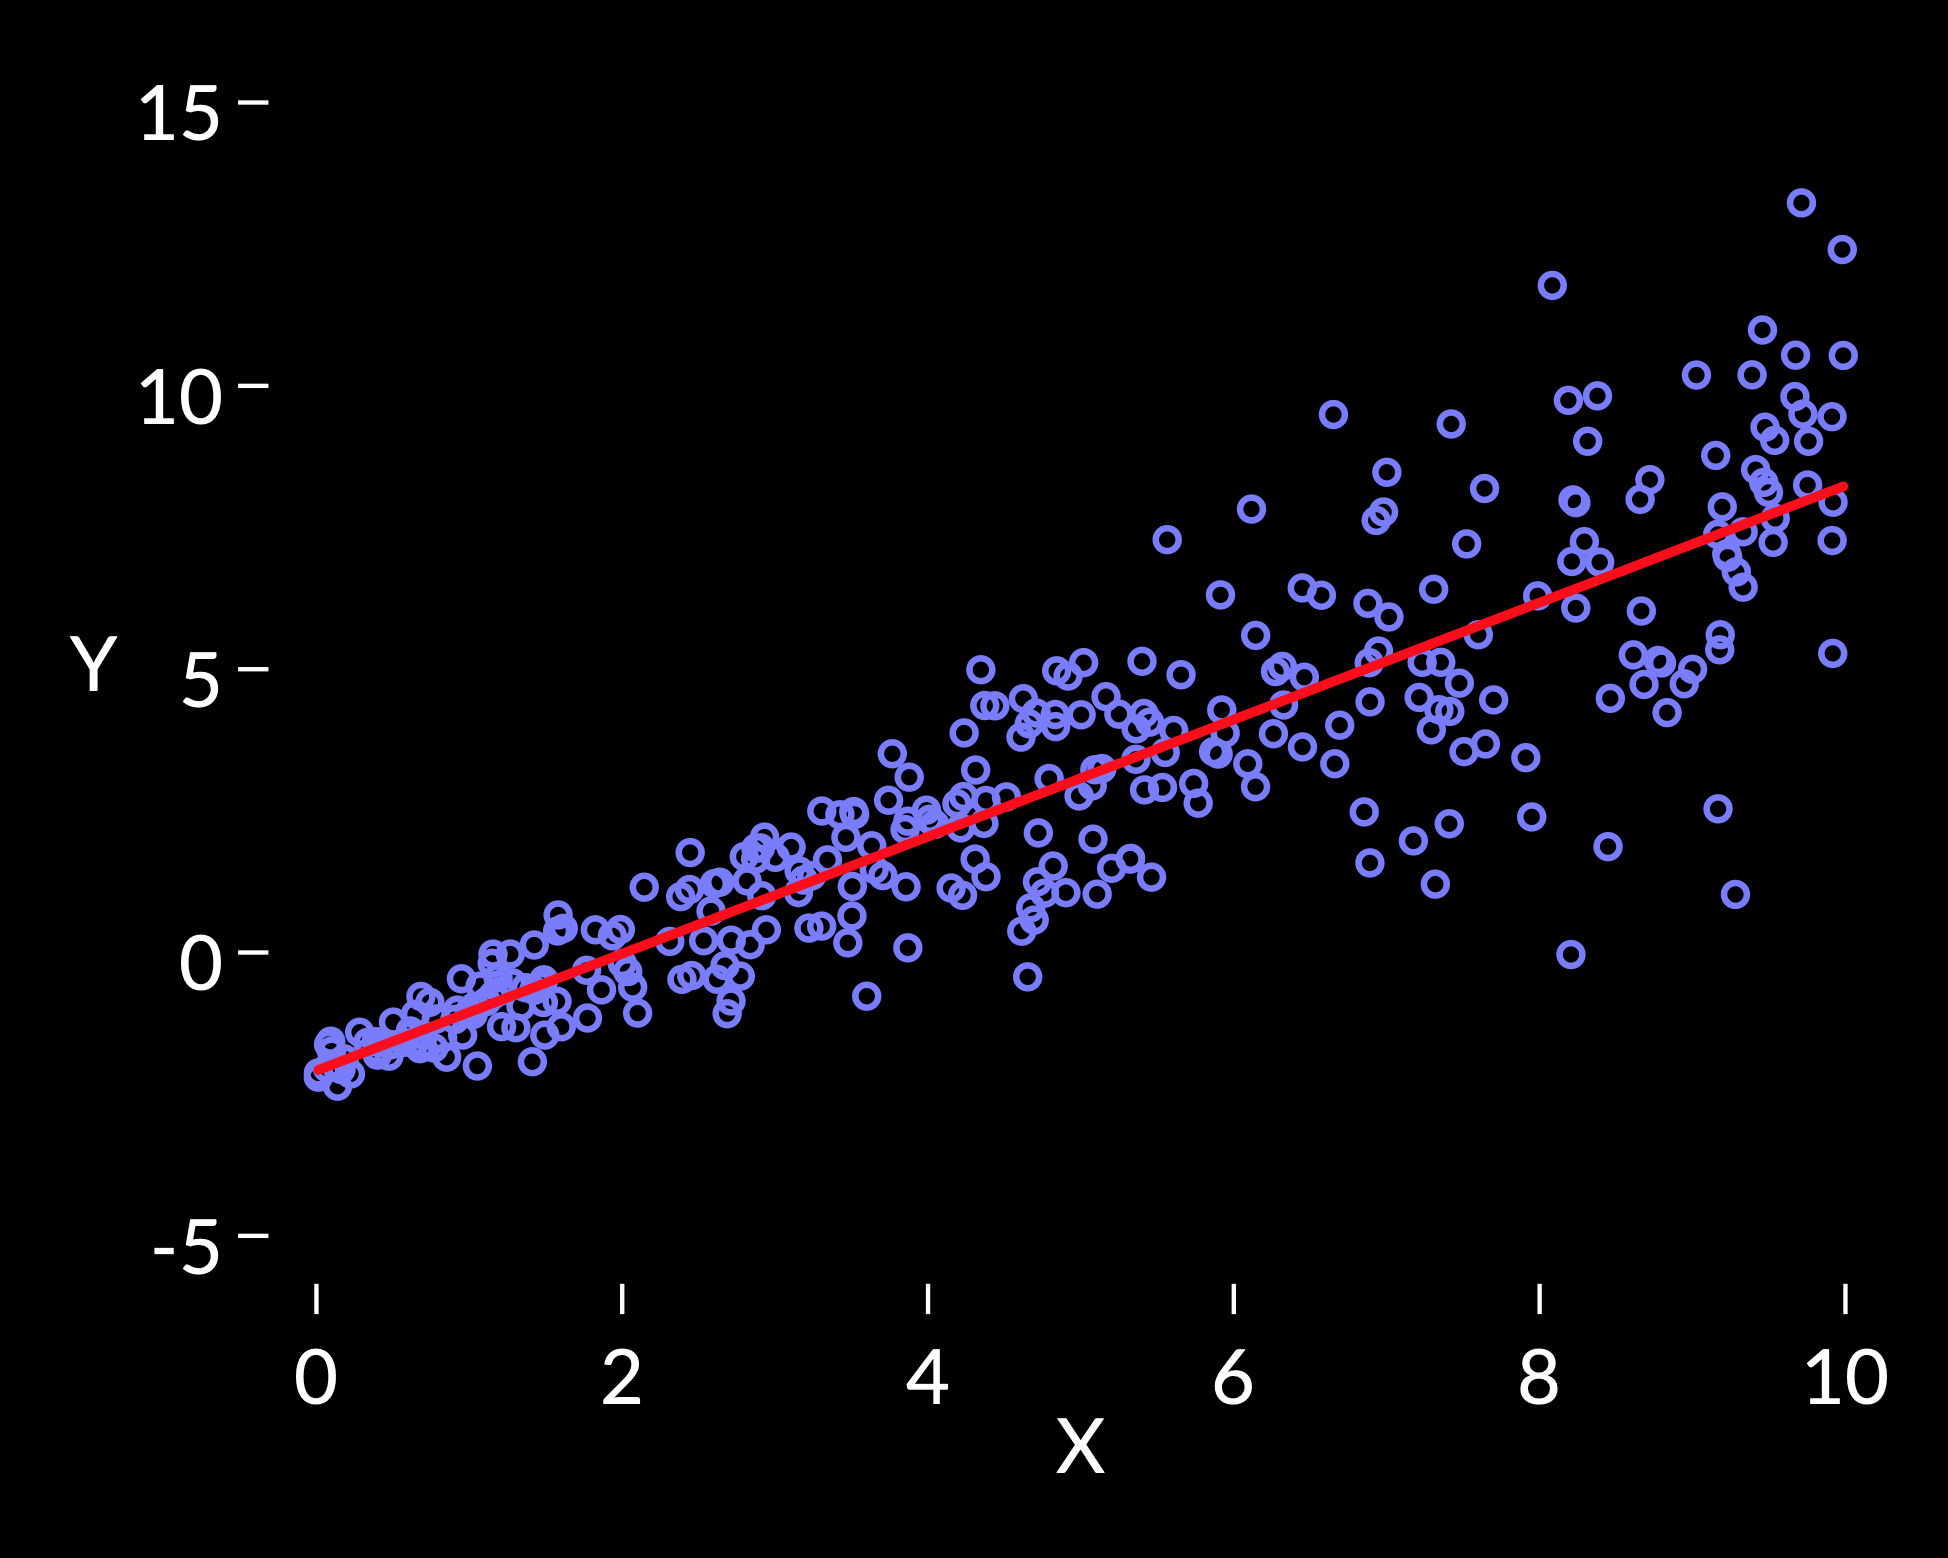
\includegraphics[width=\textwidth]{\figpath/se_hetero.png}
	\end{column}%
	\hfill%
	\begin{column}{.48\textwidth}
		\begin{witem}
		\item The macro {\textbackslash{}figpath} points to images in the
			\texttt{figs\textunderscore{}dark} directory in classroom mode
		\item But it points to \texttt{figs\textunderscore{}light} in handout mode
		\item Automate this process by using the color profiles in this template
			to create two versions of your charts
	\end{witem}
	\end{column}%
	\end{columns}
\end{frame}
	% ====================  END FRAME  ==================



	% =====================  FRAME  =====================
	% Notes go here
\InsertStataFrame{Example of two colors code here}{../code/define_colors.do}
	% =====================  FRAME  =====================


	% =====================  FRAME  =====================
	% Inline Images, Same for both
\begin{frame}
	\frametitle{Images}
	\begin{columns}[T] % align columns
	\begin{column}{.48\textwidth}
		% Source
		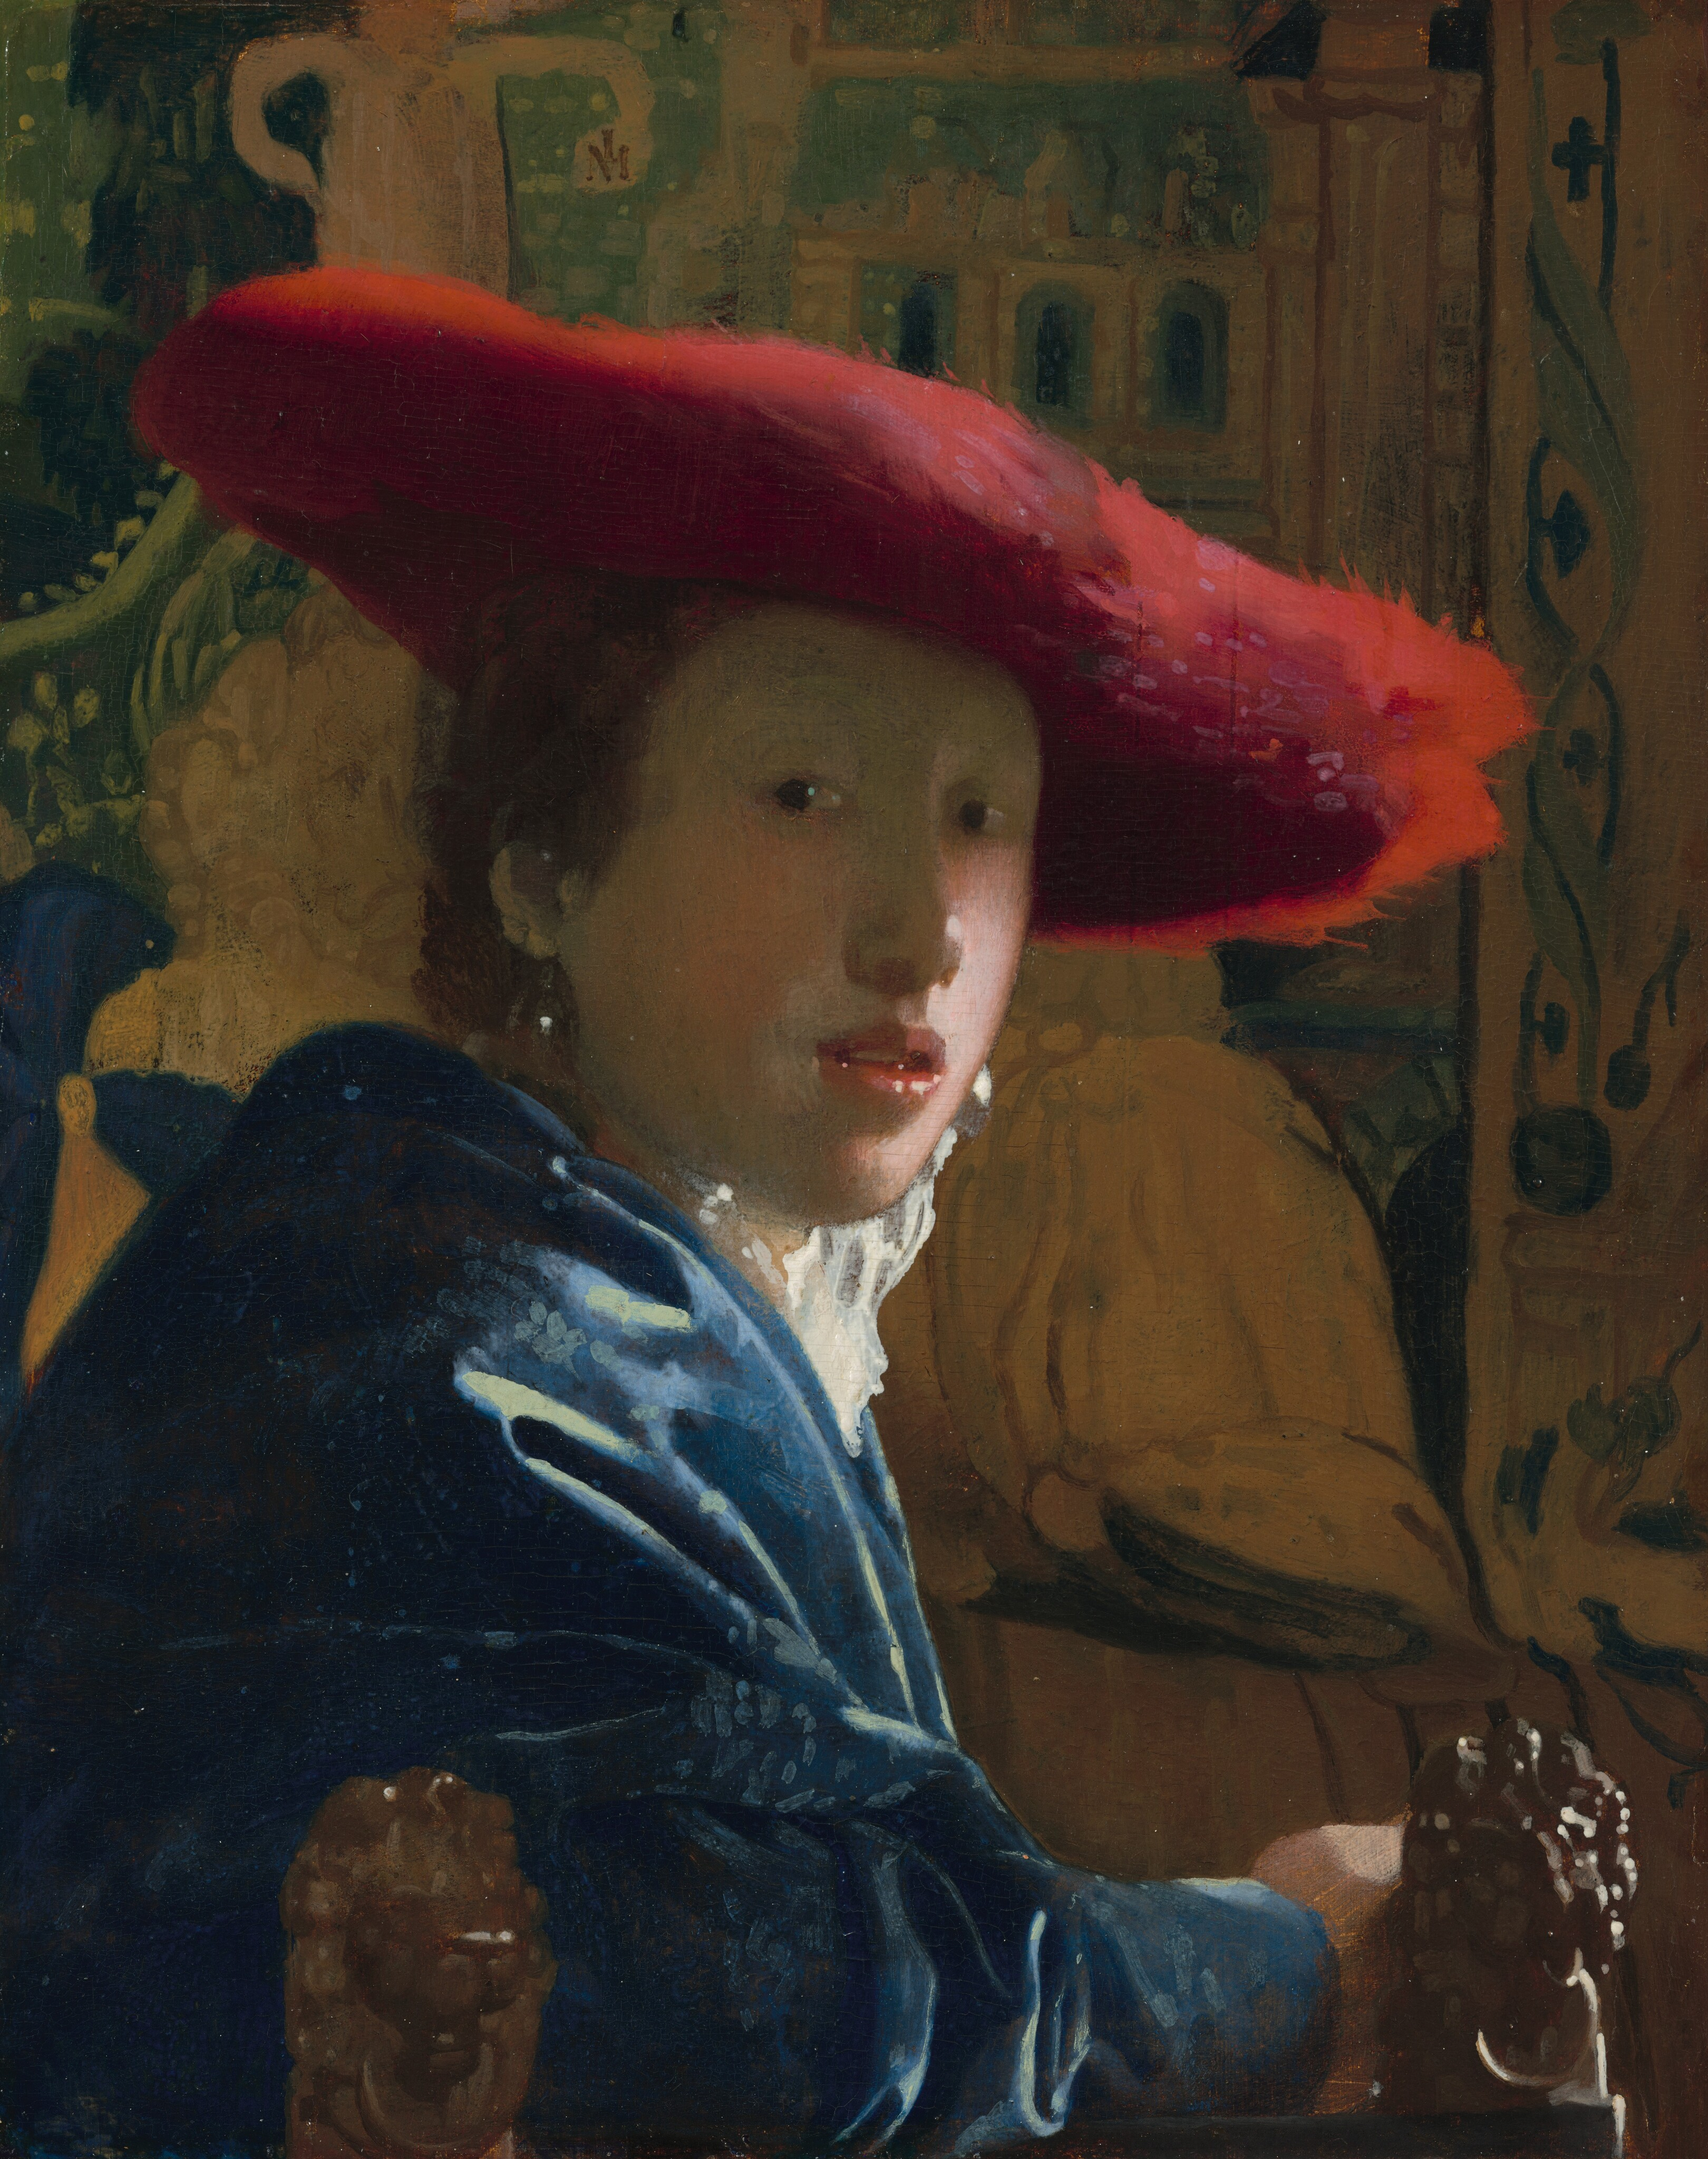
\includegraphics[width=0.9\textwidth]{\figboth/girl_with_the_red_hat_1937.1.53.jpg}
	\end{column}%
	\hfill%
	\begin{column}{.48\textwidth}
		\begin{witem}
		\item Sometimes you want to include an image that is the same for both versions
			of the slides
		\item These are stored in the \texttt{figs\textunderscore{}both} folder
		\item Use the filepath \texttt{\textbackslash{}figboth/myimage.jpg} to load the image.
	\end{witem}
	\end{column}%
	\end{columns}
\end{frame}
	% ====================  END FRAME  ==================



	% =====================  FRAME  =====================
	% Notes go here
\begin{frame}
	\frametitle{Big Images}
	\begin{witem}
		\item Sometimes, you don't want text next to your picture
		\item You want a big image you can see details of
		\item \texttt{\textbackslash{}pictureframe\{\textit{filepath}\}} will create
			a slide with one image filling as much space as it can
		\item Must be compiled twice for correct placement
	\end{witem}
\end{frame}
	% ====================  END FRAME  ==================


	% =====================  FRAME  =====================
	% Full-frame figure, differs by format
	% Image source: https://www.nga.gov/collection/art-object-page.51141.html
\pictureframe{\figpath/ratio_ols_lasso_pred.png}
	% ====================  END FRAME  ==================



	% =====================  FRAME  =====================
	% Full-frame figure, same for bothh
	% Image source: https://www.nga.gov/collection/art-object-page.51141.html
\pictureframe{\figboth/procession_by_a_lake_1969.12.2.jpg}
	% ====================  END FRAME  ==================



	% =====================  FRAME  =====================
	% Inline Images, Same for both
\begin{frame}
	\frametitle{Diagrams}
	\begin{columns}[T] % align columns
    \begin{column}{.58\textwidth}
    \begin{center}
    \resizebox{0.9\textwidth}{!}{

	  \begin{tikzpicture}[x=0.7cm,y=0.7cm]

    %\draw (-2,1.5) circle[radius=2pt]; % 
    \draw ([xshift=0pt,yshift=0pt]1.5,-1.5) node[circle, fill=xblue, inner sep=1.5pt] (X1) {$X_1$};
    
    \draw ([xshift=0pt,yshift=0pt]2,1) node[circle, fill=xblue, inner sep=1.5pt] (X2) {$X_2$};
    \draw ([xshift=0pt,yshift=0pt]-3,-1.5) node[circle, fill=xblue, inner sep=1.5pt] (X3) {$X_3$};
    \draw ([xshift=0pt,yshift=0pt]-2,3) node[circle, fill=xblue, inner sep=1.5pt] (X4) {$X_4$};

    %\draw (-1,1) node[anchor=south] {.};
    %\draw (-2,3) node[anchor=south] {.};
    %\draw (-1,2.5) node[anchor=south] {.};
    
    %\filldraw (1,3) circle[radius=2pt, fill=xred]; % {$X_0$};
    \draw ([xshift=0pt,yshift=0pt]0,0) node[circle, fill=xred, inner sep=1.5pt, visible on=<2->] (X0) {$X_0$};
    
    \draw[<->,dashed,color=xred,visible on=<2->] (X2)--(X0); % ,visible on=<2->
    \draw[<->,dotted,color=white, visible on=<2->] (X1)--(X0); % weight on x2
    \draw[<->,dashed,color=xred, visible on=<2->] (X3)--(X0); % weight on x2
    %\draw[<->,dashed,color=xred] (X4)--(X0); % weight on x2
   % \draw[<->] (0,-5)--(0,5); % l'axe des ordonnées
    %\draw[-] (-3,-2)--(3,4); % l'axe des abscisses
  \end{tikzpicture}
	}
    \end{center}
    \end{column}
	\hfill%
	\begin{column}{.48\textwidth}
		\begin{witem}
		\item If you use the theme color names, your tikz diagrams will change with the
			slide palette
		\item Overlays work! Add the \texttt{visible on} property to elements of the figure.
	\end{witem}
	\end{column}%
	\end{columns}
\end{frame}
	% ====================  END FRAME  ==================



	% =====================  FRAME  =====================
	% The end (in the classroom)
\theendframe



	% =====================  SECTION  =====================
	% Section
\transitionframe{References}
	% =====================  SECTION  ==================


	% =====================  FRAME  =====================
	% References
\begin{frame}[allowframebreaks]
	\frametitle{References}
{
\tiny
\bibliography{../bibliography.bib}{}
\bibliographystyle{aer}
}

\bigbreak
{
\tiny \color{gray}{Last update: \today{}}
}

\end{frame}
	% ====================  END FRAME  ==================





	% =====================  SECTION  =====================
	% Non-contents section
\transitionframe{Hidden Slides}
	% =====================  SECTION  =====================



	% =====================  FRAME  =====================
	% RE more math
\begin{frame}
	\frametitle{Variance of $\beta^{RE}$}\label{fr:varRE}

\begin{equation*}
				\hat{\lambda}_i = 1-\sqrt{\frac{
					\hat{\sigma}_{{\varepsilon}}^2
				}{
					T_i\hat{\sigma}_{{\nu}}^2+\hat{\sigma}_{{\varepsilon}}^2
				} }\in [0,1]
			\end{equation*}
%			\item Estimate the partially demeaned specification
			\begin{equation*}
				\left(y_{it} - \hat{\lambda}_i \ddot{y}_{it}\right)
					= \alpha^{RE}(1-\hat{\lambda}_i)
					+ \left(X_{it}-\hat{\lambda}_i\ddot{X}_{it}\right)\beta^{RE}
					+u_{it}
			\end{equation*}

%	\href{}{\beamergotobutton{Download the time-series data code}}

	\hyperlink{fr:RE_discussion}{\beamerreturnbutton{Back}}

\end{frame}
	% ====================  END FRAME  ==================




\end{document}
